\spacing{1.3}


\section{Scientific Method}
Scientists are tasked with discovering and developing the laws that govern nature using what is known as the \textbf{scientific method}.
This method consists of a series of stages common to any branch of science.
These stages are:
\begin{enumerate}[label=\numberballmDarkTeal]
        \item \textbf{Observation}.
        For example, if you try to dissolve sugar in a glass of water, you might notice that at some point the sugar no longer dissolves, no matter how much more you add.
        \item \textbf{Problem Statement}.
        The next step is to ask a series of questions.
        For instance, in the previous case, you might ask how changing the temperature, the amount of sugar, or the amount of water would affect the outcome.
        \item \textbf{Hypothesis Formulation}.
        A hypothesis is a provisional assumption made to explain a specific fact or phenomenon.
        \item \textbf{Experimentation}.
        It is necessary to carry out experimental tests to verify the hypothesis.
        \item \textbf{Analysis of Results}.
        Once experiments are conducted, you will have a set of data that must be analysed to determine whether the hypothesis is true.
        \item \textbf{Formulation of Laws, Theories, or Models}.
        Once the results are analysed, if the hypothesis is correct, it may become a law, theory, or model.
        If it is not correct, a new hypothesis must be formulated, and the method restarted from that point.
\end{enumerate}


\section{Graph Representation}
The graphical representation of experimental data is a fundamental tool in Physics and Chemistry.
Graphs allow us to visualise relationships between variables, identify trends, and analyse physical or chemical behaviour in a clear and precise manner.

Steps for correctly constructing a graph:

\begin{enumerate}[label=\numberballmDarkTeal]
        \item  Identify the variables:
        \begin{itemize}
            \item Independent variable (controlled): placed on the horizontal axis (\( X \)).
            \item Dependent variable (measured): placed on the vertical axis (\( Y \)).
        \end{itemize}
        \item Choose an appropriate scale:
        \begin{itemize}
            \item Use proportional scales that cover the full range of the data.
            \item Label the axes with regular units and values (e.g., every 2, 5, or 10 units).
        \end{itemize}
        \item Label the axes with names and units:
        \begin{itemize}
            \item Example: Temperature (°C) on the X-axis and Volume (mL) on the Y-axis.
        \end{itemize}
        \item Plot the points precisely:
        \begin{itemize}
            \item Use a ruler or software to plot the experimental points.
            \item Do not connect the points with broken lines; instead, draw a trend line or curve if appropriate.
        \end{itemize}
        \item  Add a title:
        \begin{itemize}
            \item It should reflect the relationship between the variables.
            Example: \textit{Relationship between pressure and gas volume}.
            \item Another way to name it is by stating the quantity on the \( Y \)-axis, followed by the word \( versus \), then the quantity on the \( X \)-axis.
            For example: pressure versus temperature – in this case, pressure is on the \( Y \)-axis and temperature on the \( X \)-axis.
        \end{itemize}
        \item Interpret the graph: you must indicate whether the dependence between the two quantities is directly proportional or inversely proportional (there are more types of dependence, but in this course we will only consider these two).
        \begin{itemize}
            \item \negsubro{Directly proportional}
            These are graphs shaped like straight lines of the form \( y = m\ x + n \),
            where \( y \) is the quantity on the \( Y \)-axis and \( x \) on the \( X \)-axis.
            The letter \( m \) represents the gradient (slope) and may be positive or negative.
            The letter \( n \) is the y-intercept, i.e., the point where the line crosses the x-axis.

            \begin{remark}
                If one quantity increases, the other must also increase.
            \end{remark}
            \begin{figure}[H]
                \centering
                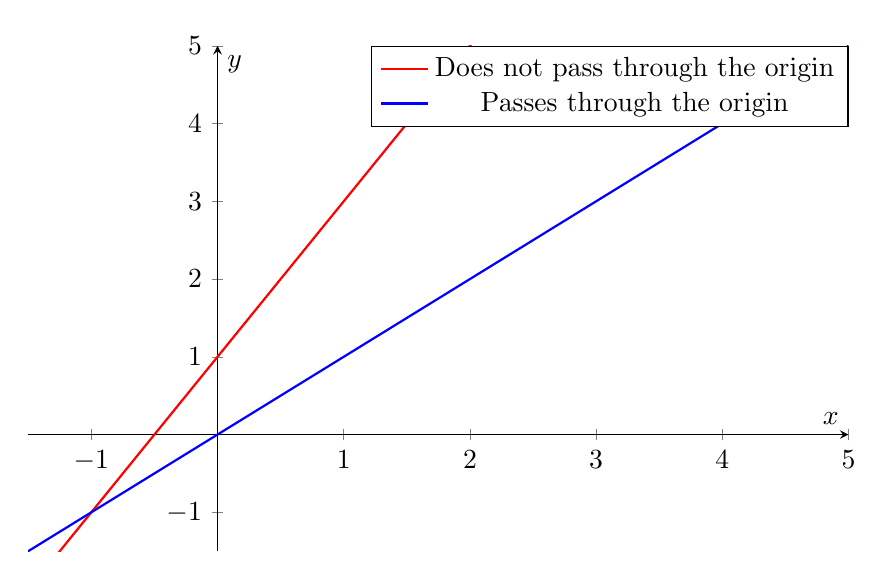
\begin{tikzpicture}
                    \begin{axis}
                        [
                        axis lines=middle,
                        xlabel={$x$},
                        ylabel={$y$},
                        xmin=-1.5, xmax=5,
                        ymin=-1.5, ymax=5,
                        legend style={at={(1,1)}, anchor=north east},
                        width=12cm,
                        height=8cm,
                        ]

                        % Line with positive gradient (y = 2x + 1)
                        \addplot[domain=-5:5, red, thick] {2*x + 1};
                        \addlegendentry{Does not pass through the origin}

                        % Line that passes through the origin (y = x)
                        \addplot[domain=-5:5, blue, thick] {x};
                        \addlegendentry{Passes through the origin}
                    \end{axis}
                \end{tikzpicture}
                \caption{Graph of two quantities that are directly proportional}
            \end{figure}
            \item \negsubro{Inversely proportional}
            These are graphs in the form of a curve like \( y = \dfrac{1}{x} \).

            \begin{remark}
                In this type of graph, if one quantity increases, the other must decrease.
            \end{remark}

            \begin{figure}[H]
                \centering
                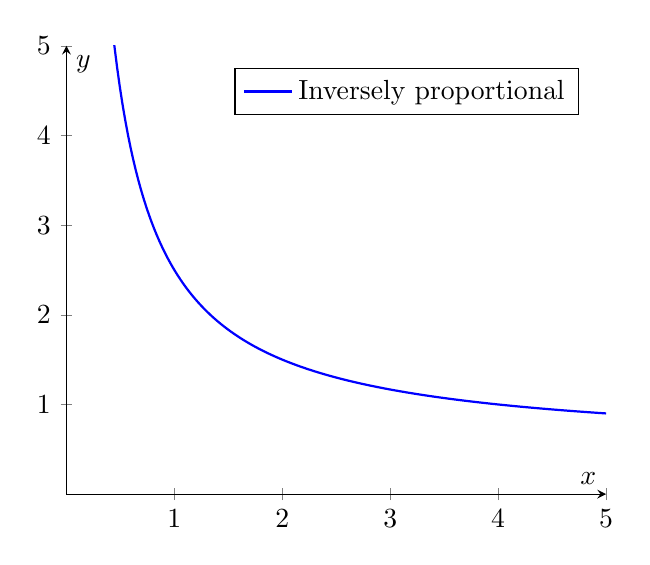
\begin{tikzpicture}
                    \begin{axis}
                        [
                        xlabel={$x$},
                        ylabel={$y$},
                        axis lines=middle,
                        ymin=0, ymax=5,
                        xmin=0, xmax=5,
                        samples=200,
                        domain=0.1:5, % Only the positive side
                        legend style={at={(0.95,0.95)}, anchor=north east},
                        legend entries={Inversely proportional}
                        ]
                        \addplot [blue, thick] {0.5 + 2/x};
                    \end{axis}
                \end{tikzpicture}
                \caption{Graph of two quantities that are inversely proportional}
            \end{figure}
        \end{itemize}
\end{enumerate}


\section{Physical Quantities and Their Units}

\begin{definition}[Physical Quantity]
        Is any property of a body that we can measure.
        By property, we mean a characteristic of an object.
\end{definition}
\vspace*{-8pt}
Every quantity, whether physical or chemical, is assigned a \textbf{unit}.
\begin{definition}[Unit]
        A unit is a quantity defined by convention to establish a standard.
\end{definition}
\vspace*{6pt}
There are several systems of units, but the most widely used is the International System of Units (SI).

It was created in 1960 by the General Conference on Weights and Measures and consists of 7 base or fundamental units.

Thanks to the SI system, the reliability of object specifications in international trade can be guaranteed.

We classify quantities into two types:

\begin{itemize}
    \item \textbf{Fundamental quantities}.
    They define these themselves; they are the basic quantities that cannot be broken down into other quantities.

    In the Table \ref{tab:magnitudes_fundamentales}, we list the fundamental quantities, their symbols, the SI units, and the unit symbols.

    % Añade en el preámbulo: \usepackage{makecell}

    \begin{table}[H]
        \centering
        \caption{Fundamental Quantities}
        \vspace{-5pt}
        \begin{tabular}{@{}lccc@{}}
            \toprule
            \textbf{Quantity} & \makecell{\textbf{Quantity} \\ \textbf{Symbol}}              & \textbf{Unit}         & \makecell{\textbf{Unit} \\ \textbf{Symbol}}                \\
            \midrule
            Length         & l         & metre   & \unit{\m} \\[3pt]
            Mass                & m         & kilogram   & \unit{\kilo\g} \\[3pt]
            Temperature    & T         & kelvin   & \unit{\kelvin} \\[3pt]
            Time & t         & second     & \unit{\s} \\[3pt]
            Electric current  & I & ampere  & \unit{\ampere} \\[3pt]
            Amount of substance  & n & mole  & \unit{\mole} \\[3pt]
            Luminous intensity  & \( I_v \) & candela  & \unit{\candela} \\
            \bottomrule
        \end{tabular}
        \label{tab:magnitudes_fundamentales}
    \end{table}

%    \begin{table}[H]
%        \centering
%        \caption{Fundamental quantities}
%        \label{table:fundamental_quantities}
%        \begin{tblr}
%        {
%            colspec={|c|c|c|c|},
%            row{1} = {bg=darkblue!80, fg=white, font=\bfseries},
%            hlines,
%            vlines
%        }
%            Quantity & Quantity Symbol & Unit & Unit Symbol \\
%            Length & l & metre & \unit{\m} \\
%            Mass & m & kilogram & \unit{\kilo\g} \\
%            Temperature & T & kelvin & \unit{\kelvin} \\
%            Time & t & second & \unit{\s} \\
%            Electric current & I & ampere & \unit{\ampere} \\
%            Amount of substance & n & mole & \unit{\mole} \\
%            Luminous intensity & \( I_v \) & candela & \unit{\candela} \\
%        \end{tblr}
%    \end{table}


    \item \textbf{Derived quantities}.
    These are formed from the fundamental quantities and can be expressed as combinations of them.

    Table \ref{tab:derivative_quantities} lists some derived quantities with their units in the International System.

    \begin{table}[H]
        \centering
        \caption{Derived Quantities}
        \vspace{-5pt}
        \begin{tabular}{@{}lccc@{}}
            \toprule
            \textbf{Quantity} & \makecell{\textbf{Quantity} \\ \textbf{Symbol}}     & \textbf{Unit}          & \makecell{\textbf{Unit} \\ \textbf{Symbol}}   \\
            \midrule
            Area  & A & square metre           & \unit{\square\m} \\[3pt]
            Volume    & V          & cubic metre           & \unit{\cubic\m} \\[3pt]
            Density    & \( \rho \)          & --       & \unit{\kilo\g\per\cubic\m} \\[3pt]
            Speed & v          & --       & \unit{\mps} \\[3pt]
            Force   & F          & newton        & \unit{\newton} \\[3pt]
            Pressure   & p          & pascal        & \unit{\pascal} \\[3pt]
            Energy   & E          & joule        & \unit{\joule} \\[3pt]
            \bottomrule
        \end{tabular}
        \label{tab:derivative_quantities}
    \end{table}

%    \begin{table}[H]
%        \centering
%        \caption{Derivative quantities}
%        \label{table:derivative_quantities}
%        \begin{tblr}{
%            colspec={|c|c|c|c|},
%            row{1} = {bg=darkblue!80, fg=white, font=\bfseries},
%            hlines,
%            vlines
%        }
%            Quantity & Quantity Symbol & Unit & Unit Symbol \\
%            Area & A & square metre & \unit{\square\m} \\
%            Volume & V & cubic metre & \unit{\cubic\m} \\
%            Density & \( \rho \) & -- & \unit{\kilo\g\per\cubic\m} \\
%            Speed & v & -- & \unit{\mps} \\
%            Force & F & newton & \unit{\newton} \\
%            Pressure & p & pascal & \unit{\pascal} \\
%            Energy & E & joule & \unit{\joule} \\
%        \end{tblr}
%    \end{table}
\end{itemize}

\begin{remark}
    If we want to determine whether a quantity is fundamental or derived, the simplest method is to learn the fundamental ones.
    If it is not fundamental, then it is derived.
\end{remark}

\begin{exercise}
    In your notebook, indicate which of the following quantities are fundamental and which are derived:
    \vspace*{-12pt}
    \begin{multicols}{3}
        \begin{enumerate}[label=\letraminuscula]
            \item Electric current.
            \item Pressure.
            \item Speed.
            \item Mass.
            \item Temperature.
            \item Density.
            \item Energy.
            \item Length.
            \item Amount of substance
        \end{enumerate}
    \end{multicols}
    \begin{solu}
        In your notebook, indicate which of the following quantities are fundamental and which are derived:
        \begin{multicols}{2}
            \begin{enumerate}[label=\letraminuscula]
            \item Electric current. \textcolor{ocre}{Derived}
            \item Pressure. \textcolor{ocre}{Derived}
            \item Speed. \textcolor{ocre}{Derived}
            \item Mass. \textcolor{ocre}{Fundamental}
            \item Temperature. \textcolor{ocre}{Fundamental}
            \item Density. \textcolor{ocre}{Derived}
            \item Energy.\textcolor{ocre}{Derived}
            \item Length. \textcolor{ocre}{Fundamental}
            \end{enumerate}
        \end{multicols}
    \end{solu}
\end{exercise}

\subsection{Multiples and Submultiples}

When defining a system of units, it is also necessary to establish the multiples and submultiples of these units, which allow us to work with more manageable numerical quantities.

The following table shows the relationship between a unit and the various proportionality factors corresponding to its multiples and submultiples.
\begin{multicols}{2}
    \begin{table}[H]
        \centering
        \caption{Multiples}
        \vspace{-5pt}
        \begin{tabular}{@{}ccc@{}}
            \toprule
            \textbf{Order of Magnitude} & \textbf{Name} & \textbf{Symbol} \\
            \midrule
            \num{e12}                   & tera-         & T     \\[3pt]
            \num{e9}                    & giga-         & G               \\[3pt]
            \num{e6}                    & mega-         & M               \\[3pt]
            \num{e3}                    & kilo-         & k               \\[3pt]
            \num{e2}                    & hecto-        & h               \\[3pt]
            \num{10}                    & deca-         & da              \\[3pt]
            \bottomrule
            \multicolumn{3}{c}{\textbf{Base Unit} }
            \\
            \bottomrule
        \end{tabular}
        \label{tab:Multiples}
    \end{table}
%    \begin{table}[H]
%        \caption{Multiples}
%        \label{table:Multiples}
%        \begin{tblr}{
%            colspec={|c|c|c|},
%            row{1} = {bg=darkblue!80, fg=white, font=\bfseries},
%            hlines,
%            vlines
%        }
%            Order of Magnitude & Name  & Symbol \\
%            \num{e12} & tera- & T \\
%            \num{e9} & giga- & G \\
%            \num{e6} & mega- & M \\
%            \num{e3} & kilo- & k \\
%            \num{e2} & hecto- & h \\
%            \num{10} & deca- & da \\
%            \SetRow{darkblue!70}\SetCell[c=3]{c} \textbf{\textcolor{white}{Base Unit}}
%        \end{tblr}
%    \end{table}
    \columnbreak
    \begin{table}[H]
        \centering
        \caption{Submultiples}
        \vspace{-5pt}
        \begin{tabular}{@{}ccc@{}}
            \toprule
            \textbf{Order of Magnitude} & \textbf{Name} & \textbf{Symbol} \\
            \toprule
            \multicolumn{3}{c}{\textbf{Base Unit} } \\
            \toprule
            \num{e-1}                   & deci-         & d \\[3pt]
            \num{e-2}                   & centi-        & c \\[3pt]
            \num{e-3}                   & milli-        & m \\[3pt]
            \num{e-6}                   & micro-        & \( \mu \) \\[3pt]
            \num{e-9}                   & nano-         & n \\[3pt]
            \num{e-12}                  & pico-         & p               \\
            \bottomrule
        \end{tabular}
        \label{tab:Submultiples}
    \end{table}
%    \begin{table}[H]
%        \caption{Submultiples}
%        \label{table:Submultiples}
%
%        \begin{tblr}{
%            colspec={|c|c|c|},
%            row{1} = {bg=darkblue!80, fg=white, font=\bfseries},
%            hlines,
%            vlines
%        }
%            Order of Magnitude & Name  & Symbol \\
%            \SetRow{darkblue!70}\SetCell[c=3]{c} \textbf{\textcolor{white}{Base Unit}} \\
%            \num{e-1} & deci- & d \\
%            \num{e-2} & centi- & c \\
%            \num{e-3} & milli- & m \\
%            \num{e-6} & micro- & \( \mu \) \\
%            \num{e-9} & nano- & n \\
%            \num{e-12} & pico- & p \\
%        \end{tblr}
%    \end{table}
\end{multicols}

SI units are not the only ones in use; in fact, almost every quantity has several possible units.
The following table lists quantities with various units and their equivalences with other units of the same quantity.

\begin{table}[H]
    \centering
    \caption{Quantities with their equivalences}
    \vspace{-5pt}
    \begin{tabular}{@{}ccc@{}}
        \toprule
        \textbf{Quantity}         & \textbf{Unit}                   & \textbf{Unit Equivalence}                           \\
        \midrule
        \multirow{3}{*}{Volume}   & \unit{\kilo\litre}              & \qty{1}{\kilo\litre} = \qty{1}{\cubic\metre}        \\[3pt]
        & \unit{\litre}                   & \qty{1}{\litre} = \qty{1}{\cubic\deci\metre}        \\[3pt]
        & \unit{\milli\litre}             & \qty{1}{\milli\litre} = \qty{1}{\cubic\centi\metre} \\[3pt]
        \midrule
        \multirow{3}{*}{Pressure} & Atmosphere (\unit{\atmosphere}) & \qty{1}{\atmosphere} = \qty{e5}{\pascal} \\[3pt]
        & \makecell{millimetre of mercury \\  (\unit{\mmHg})}                    & \qty{1}{\atmosphere} = \qty{760}{\mmHg} \\[3pt]
        \midrule
        Energy                     & Calorie (\unit{\cal})           & \qty{1}{\cal} = \qty{4.18}{\joule}                   \\[3pt]
        \midrule
        Force                     & Kilopond (\unit{\kp})           & \qty{1}{\kp} = \qty{9.8}{\newton}                   \\
        \bottomrule
    \end{tabular}
    \label{tab:quantities_with_their_equivalences}
\end{table}

%\begin{table}[H]
%    \centering
%    \caption{Quantities with their equivalences}
%    \label{table:quantities_with_their_equivalences}
%    \begin{tblr}{
%        colspec={|c|c|c|},
%        row{1} = {bg=darkblue!80, fg=white, font=\bfseries},
%        hlines,
%        vlines,
%        cell{2}{1}={r=3}{c},
%        cell{5}{1}={r=2}{c},
%        rowhead=1
%    }
%        Quantity & Unit & Unit Equivalence \\
%        Volume & \unit{\kilo\litre} & \qty{1}{\kilo\litre} = \qty{1}{\cubic\metre} \\
%        & \unit{\litre} & \qty{1}{\litre} = \qty{1}{\cubic\deci\metre} \\
%        & \unit{\milli\litre} & \qty{1}{\milli\litre} = \qty{1}{\cubic\centi\metre} \\
%        Pressure & {Atmosphere \\ (\unit{\atmosphere})} & \qty{1}{\atmosphere} = \qty{e5}{\pascal} \\
%        & {millimetre of mercury \\ (\unit{\mmHg})} & \qty{1}{\atmosphere} = \qty{760}{\mmHg} \\
%        Energy & Calorie (\unit{\cal}) & \qty{1}{\cal} = \qty{4.18}{\joule} \\
%        Force & Kilopond (\unit{\kp}) & \qty{1}{\kp} = \qty{9.8}{\newton} \\
%    \end{tblr}
%\end{table}

\subsection{Converting Units Using Conversion Factors}

We must first keep the following in mind:
\begin{enumerate}[label=\letraminuscula]
        \item We can convert between units as long as they belong to the same quantity.
        \item We can convert between units with different multiples and submultiples.
        \item We can also convert between different units as long as they represent the same quantity, and we know the equivalence between them.
\end{enumerate}

\begin{example}
    Let us convert \qty{36}{\kmph} to \unit{\mps}:
    \begin{equation*}
        36\ \dfrac{\cancelred{\unit{\kilo\metre}}}{\cancel{\unit{\hour}}} \cdot \dfrac{1000\ \unit{\metre}}{1\ \cancelred{\unit{\kilo\metre}}} \cdot \dfrac{1\ \cancelred{\unit{\hour}}}{3600\ \unit{\second}} = \dfrac{36 \cdot 1000}{3600} = \qty{10}{\mps}
    \end{equation*}
\end{example}

\begin{example}
    Convert \qty{13600}{\kilo\g\per\cubic\metre} to \unit{\g\per\cubic\centi\metre}:
    \begin{equation*}
        13600\ \dfrac{\cancelred{\unit{\kilo\g}}}{\cancel{\unit{\cubic\metre}}} \cdot \dfrac{1000\ \unit{\g}}{1\ \cancelred{\unit{\kilo\g}}} \cdot \dfrac{1\ \cancelred{\unit{\cubic\metre}}}{\num{e6}\ \unit{\cubic\centi\metre}} = \dfrac{13600 \cdot 1000}{\num{e6}} = \qty{13.6}{\g\per\cubic\centi\metre}
    \end{equation*}
\end{example}

\begin{example}
    Convert \qty{12}{\kilo\metre} to \unit{\nano\metre}:
    \begin{equation*}
        12\ \cancelred{\unit{\kilo\metre}} \cdot  \dfrac{\num{e12}\ \unit{\nano\metre}}{ 1\ \cancelred{\unit{\kilo\metre}}} = \num{12e-12} = \qty{1.2e-11}{\nano\metre}
    \end{equation*}
\end{example}

\begin{exercise}
    Convert the following speeds into the indicated units using conversion factors.
    \begin{enumerate}[label=\letraminuscula]
        \item Convert the following speeds into \unit{\mps}:
        \begin{multicols}{4}
            \begin{itemize}
                \item \qty{90}{\kmph}
                \item \qty{100}{\kmph}
                \item \qty{120}{\kmph}
                \item \qty{50}{\kmph}
            \end{itemize}
        \end{multicols}
        \item Convert the following speeds into \unit{\kmph}:
        \begin{multicols}{4}
            \begin{itemize}
                \item \qty{12}{\mps}
                \item \qty{340}{\mps}
                \item \qty{0.36}{\mps}
                \item \qty{3e8}{\mps}
            \end{itemize}
        \end{multicols}
    \end{enumerate}
    \begin{solu}

        To perform these conversions, we use the following equivalence relations: $1 \text{ km} = 1000 \text{ m}$ and $1 \text{ h} = 3600 \text{ s}$.

        \textbf{a) Conversion from km/h to m/s:}
        \begin{itemize}
            \item \textbf{90 km/h}:
            \[ 90 \frac{\cancel{\text{km}}}{\cancel{\text{h}}} \cdot \frac{1000 \text{ m}}{1 \cancel{\text{km}}} \cdot \frac{1 \cancel{\text{h}}}{3600 \text{ s}} = \frac{90 \cdot 1000}{3600} \text{ m/s} = 25 \text{ m/s} \]

            \item \textbf{100 km/h}:
            \[ 100 \frac{\cancel{\text{km}}}{\cancel{\text{h}}} \cdot \frac{1000 \text{ m}}{1 \cancel{\text{km}}} \cdot \frac{1 \cancel{\text{h}}}{3600 \text{ s}} = \frac{100000}{3600} \text{ m/s} \approx 27.78 \text{ m/s} \]

            \item \textbf{120 km/h}:
            \[ 120 \frac{\cancel{\text{km}}}{\cancel{\text{h}}} \cdot \frac{1000 \text{ m}}{1 \cancel{\text{km}}} \cdot \frac{1 \cancel{\text{h}}}{3600 \text{ s}} = \frac{120000}{3600} \text{ m/s} \approx 33.33 \text{ m/s} \]

            \item \textbf{50 km/h}:
            \[ 50 \frac{\cancel{\text{km}}}{\cancel{\text{h}}} \cdot \frac{1000 \text{ m}}{1 \cancel{\text{km}}} \cdot \frac{1 \cancel{\text{h}}}{3600 \text{ s}} = \frac{50000}{3600} \text{ m/s} \approx 13.89 \text{ m/s} \]
        \end{itemize}

        \textbf{b) Conversion from m/s to km/h:}
        \begin{itemize}
            \item \textbf{12 m/s}:
            \[ 12 \frac{\cancel{\text{m}}}{\cancel{\text{s}}} \cdot \frac{1 \text{ km}}{1000 \cancel{\text{m}}} \cdot \frac{3600 \cancel{\text{s}}}{1 \text{ h}} = 12 \cdot 3.6 \text{ km/h} = 43.2 \text{ km/h} \]

            \item \textbf{340 m/s}:
            \[ 340 \frac{\cancel{\text{m}}}{\cancel{\text{s}}} \cdot \frac{1 \text{ km}}{1000 \cancel{\text{m}}} \cdot \frac{3600 \cancel{\text{s}}}{1 \text{ h}} = 340 \cdot 3.6 \text{ km/h} = 1224 \text{ km/h} \]

            \item \textbf{0.36 m/s}:
            \[ 0.36 \frac{\cancel{\text{m}}}{\cancel{\text{s}}} \cdot \frac{1 \text{ km}}{1000 \cancel{\text{m}}} \cdot \frac{3600 \cancel{\text{s}}}{1 \text{ h}} = 0.36 \cdot 3.6 \text{ km/h} = 1.296 \text{ km/h} \]

            \item \textbf{$3 \cdot 10^8$ m/s}:
            \[ 3 \cdot 10^8 \frac{\cancel{\text{m}}}{\cancel{\text{s}}} \cdot \frac{1 \text{ km}}{1000 \cancel{\text{m}}} \cdot \frac{3600 \cancel{\text{s}}}{1 \text{ h}} = 3 \cdot 10^8 \cdot 3.6 \text{ km/h} = 1.08 \cdot 10^9 \text{ km/h} \]
        \end{itemize}
    \end{solu}
\end{exercise}


\begin{exercise}
    Convert the following units into the corresponding SI units using conversion factors.
    \begin{multicols}{4}
        \begin{enumerate}[label=\letraminuscula]
            \item \qty{200}{\square\centi\metre}
            \item \qty{125}{\cubic\centi\metre}
            \item \qty{1800}{\g}
            \item \qty{45}{\min}
        \end{enumerate}
    \end{multicols}


    \begin{solu}
        To convert these values to the International System of Units (SI), we use the base units: meters (\unit{\m}), kilograms (\unit{\kg}), and seconds (\unit{\s}).

        \textbf{a) Area conversion (\unit{\square\centi\metre} to \unit{\square\metre}):}
        Since \( \qty{1}{\metre} = \qty{100}{\centi\metre} \), then \( \qty{1}{\square\metre} = (\qty{100}{\centi\metre})^2 = \qty{10000}{\square\centi\metre} \).
        \[ \qty{200}{\cancel{\square\centi\metre}} \cdot \frac{\qty{1}{\square\metre}}{\qty{10000}{\cancel{\square\centi\metre}}} = \qty{0.02}{\square\metre} \]

        \textbf{b) Volume conversion (\unit{\cubic\centi\metre} to \unit{\cubic\metre}):}
        Since \( \qty{1}{\metre} = \qty{100}{\centi\metre} \), then \( \qty{1}{\cubic\metre} = (\qty{100}{\centi\metre})^3 = \qty{1000000}{\cubic\centi\metre} \).
        \[ \qty{125}{\cancel{\cubic\centi\metre}} \cdot \frac{\qty{1}{\cubic\metre}}{\qty{1000000}{\cancel{\cubic\centi\metre}}} = \qty{1.25e-4}{\cubic\metre} \]

        \textbf{c) Mass conversion (\unit{\g} to \unit{\kg}):}
        Equivalence: \( \qty{1}{\kg} = \qty{1000}{\g} \).
        \[ \qty{1800}{\cancel{\g}} \cdot \frac{\qty{1}{\kg}}{\qty{1000}{\cancel{\g}}} = \qty{1.8}{\kg} \]

        \textbf{d) Time conversion (\unit{\min} to \unit{\s}):}
        Equivalence: \( \qty{1}{\min} = \qty{60}{\s} \).
        \[ \qty{45}{\cancel{\min}} \cdot \frac{\qty{60}{\s}}{\qty{1}{\cancel{\min}}} = \qty{2700}{\s} \]
    \end{solu}

\end{exercise}

\begin{exercise}
    Perform the following unit conversions into SI units using conversion factors
    \begin{multicols}{4}
        \begin{enumerate}[label=\letraminuscula]
\item \qty{300}{\mmHg}
\item \qty{25000}{\cal}
\item \qty{21}{\atmosphere}
\item \qty{258}{\kilopondio}
        \end{enumerate}
    \end{multicols}


    \begin{solu}
        In the International System, the derived unit for pressure is the Pascal (\unit{\Pa}), for energy it is the Joule (\unit{\J}), and for force it is the Newton (\unit{\N}).

        \textbf{a) Pressure (\unit{\mmHg} to \unit{\Pa}):}
        Equivalence: \( \qty{760}{\mmHg} = \qty{101325}{\Pa} \).
        \[ \qty{300}{\cancel{\mmHg}} \cdot \frac{\qty{101325}{\Pa}}{\qty{760}{\cancel{\mmHg}}} \approx \qty{39996.71}{\Pa} \]

        \textbf{b) Energy (\unit{cal} to \unit{\J}):}
        Equivalence: \( \qty{1}{cal} = \qty{4.184}{\J} \).
        \[ \qty{25000}{\cancel{cal}} \cdot \frac{\qty{4.184}{\J}}{\qty{1}{\cancel{cal}}} = \qty{104600}{\J} \]

        \textbf{c) Pressure (\unit{atm} to \unit{\Pa}):}
        Equivalence: \( \qty{1}{atm} = \qty{101325}{\Pa} \).
        \[ \qty{21}{\cancel{atm}} \cdot \frac{\qty{101325}{\Pa}}{\qty{1}{\cancel{atm}}} = \qty{2127825}{\Pa} \]

        \textbf{d) Force (\unit{kp} to \unit{\N}):}
        Equivalence: \( \qty{1}{kp} = \qty{9.8}{\N} \).
        \[ \qty{258}{\cancel{kp}} \cdot \frac{\qty{9.8}{\N}}{\qty{1}{\cancel{kp}}} = \qty{2528.4}{\N} \]
    \end{solu}

\end{exercise}

\begin{exercise}
    If 1 g of pure gold costs 31.32 €, calculate the price of 1 dg and 1 cg of this metal. Resolve the following exercise using factor conversion.

    \begin{solu}
        Using the mass relationships within the decimal system: \( \qty{1}{\g} = \qty{10}{\deci\g} \) and \( \qty{1}{\g} = \qty{100}{\centi\g} \).

        \textbf{1) Price for \qty{1}{\deci\g}:}
        \[ \qty{1}{\cancel{\deci\g}} \cdot \frac{\qty{1}{\cancel{\g}}}{\qty{10}{\cancel{\deci\g}}} \cdot \frac{\text{31.32 €}}{\qty{1}{\cancel{\g}}} = \text{3.13 €} \]

        \textbf{2) Price for \qty{1}{\centi\g}:}
        \[ \qty{1}{\cancel{\centi\g}} \cdot \frac{\qty{1}{\cancel{\g}}}{\qty{100}{\cancel{\centi\g}}} \cdot \frac{\text{31.32 €}}{\qty{1}{\cancel{\g}}} = \text{0.31 €} \]
    \end{solu}

\end{exercise}

\begin{exercise}
    If 1 kg of almonds costs 18.40 €, calculate the price of 1 hg and 1 dag of this product. Resolve the following exercise using factor conversion.

    \begin{solu}
        Using the mass relationships within the decimal system: \( \qty{1}{\kg} = \qty{10}{\hecto\g} \) and \( \qty{1}{\kg} = \qty{100}{\deca\g} \).

        \textbf{1) Price for \qty{1}{\hecto\g}:}
        \[
        \qty{1}{\cancel{\hecto\g}} \cdot
        \frac{\qty{1}{\cancel{\kg}}}{\qty{10}{\cancel{\hecto\g}}} \cdot
        \frac{\text{18.40 €}}{\qty{1}{\cancel{\kg}}}
        = \text{1.84 €}
        \]

        \textbf{2) Price for \qty{1}{\deca\g}:}
        \[
        \qty{1}{\cancel{\deca\g}} \cdot
        \frac{\qty{1}{\cancel{\kg}}}{\qty{100}{\cancel{\deca\g}}} \cdot
        \frac{\text{18.40 €}}{\qty{1}{\cancel{\kg}}}
        = \text{0.184 €}
        \]
    \end{solu}

\end{exercise}

\begin{exercise}
    If 1 L of olive oil costs 9.60 €, calculate the price of 1 dL and 1 cL of this liquid. Resolve the following exercise using factor conversion.

    \begin{solu}
        Using the capacity relationships within the decimal system: \( \qty{1}{\L} = \qty{10}{\deci\L} \) and \( \qty{1}{\L} = \qty{100}{\centi\L} \).

        \textbf{1) Price for \qty{1}{\deci\L}:}
        \[
        \qty{1}{\cancel{\deci\L}} \cdot
        \frac{\qty{1}{\cancel{\L}}}{\qty{10}{\cancel{\deci\L}}} \cdot
        \frac{\text{9.60 €}}{\qty{1}{\cancel{\L}}}
        = \text{0.96 €}
        \]

        \textbf{2) Price for \qty{1}{\centi\L}:}
        \[
        \qty{1}{\cancel{\centi\L}} \cdot
        \frac{\qty{1}{\cancel{\L}}}{\qty{100}{\cancel{\centi\L}}} \cdot
        \frac{\text{9.60 €}}{\qty{1}{\cancel{\L}}}
        = \text{0.096 €}
        \]
    \end{solu}

\end{exercise}


\section{Scientific Notation}

Scientific notation allows us to write huge or tiny numbers using powers of \num{10}, with a positive exponent for huge numbers or a negative exponent for tiny ones.

For a number to be correctly expressed in scientific notation, it must have:

\begin{itemize}
    \item A single non-zero digit to the left of the decimal point.
    \item A power of 10 raised to a positive or negative exponent.
\end{itemize}

For example:

\begin{itemize}
    \item The mass of the Earth is:

    \qty{6000000000000000000000000}{\kilo\g}.
    As we can see, this number has 24 zeros, so writing it repeatedly is quite tedious.
    This number in scientific notation would be: \qty{6e24}{\kilo\g}.

    \item The mass of the electron is:

    \qty{0.0000000000000000000000000000009109}{\kilo\g}.
    This number in scientific notation is written as \qty{9.3109e-31}{\kilo\g}.
\end{itemize}

The steps for converting to scientific notation are as follows:

\begin{itemize}
    \item \textbf{Numbers greater than one}.
    Start at the right of the number.
    At that point, we place the decimal point and count how many positions we need to move it so that only one non-zero digit remains to its left.
    The number in scientific notation will be the new number multiplied by a power of 10, raised to the number of positions moved, with a positive exponent.
    That’s why in the earlier case we get \num{6e24}.

    \item \textbf{Numbers smaller than one}.
    We start at the decimal point and count how many positions we need to move it so that there is only one non-zero digit to its left.
    The resulting exponent will be negative.

    \item \textbf{Numbers that are already large or small but already include a power of 10} .
    We begin at the decimal point.
    The following cases may occur:

    \begin{itemize}
        \item If the number is greater than one:
        We proceed as in the previous case, and the number of positions is \emph{added} to the exponent of the decimal. Examples:
        \begin{itemize}
            \item \num{625.5e5} becomes \num{6.255e7}.
            \item \num{45654.21e-2} becomes \num{4.5654e-2}.
        \end{itemize}

        \item If the number is smaller than one:
        We proceed similarly, but in this case the number of positions is \emph{subtracted} from the exponent. Examples:
        \begin{itemize}
            \item \num{0.0523e-3} becomes \num{5.23e-5}.
            \item \num{0.000254e5} becomes \num{2.54e-1}.
        \end{itemize}
    \end{itemize}
\end{itemize}

\begin{exercise}
    Write the following quantities in scientific notation:
    \begin{multicols}{3}
        \begin{enumerate}[label=\letraminuscula]
\item \qty{20000000}{\m}
\item \qty{250000000}{\litre}
\item \qty{7820000000}{\g}
\item \qty{254830368}{\km}
\item \qty{0.0001}{\s}
\item \qty{0.000035}{\kilo\g}
\item \qty{0.000001}{\m}
\item \qty{0.000005001}{\g}
\item \qty{0.000000005}{\g}
        \end{enumerate}
    \end{multicols}

    \begin{solu}
        To write in scientific notation, we move the decimal point to create a number between 1 and 10, then multiply by the corresponding power of 10.
        \begin{itemize}
            \item \textbf{a)} \( \qty{20000000}{\m} = \qty{2e7}{\m} \)
            \item \textbf{b)} \( \qty{250000000}{\litre} = \qty{2.5e8}{\litre} \)
            \item \textbf{c)} \( \qty{7820000000}{\g} = \qty{7.82e9}{\g} \)
            \item \textbf{d)} \( \qty{254830368}{\km} \approx \qty{2.55e8}{\km} \)
            \item \textbf{e)} \( \qty{0.0001}{\s} = \qty{1e-4}{\s} \)
            \item \textbf{f)} \( \qty{0.000035}{\kg} = \qty{3.5e-5}{\kg} \)
            \item \textbf{g)} \( \qty{0.000001}{\m} = \qty{1e-6}{\m} \)
            \item \textbf{h)} \( \qty{0.000005001}{\g} = \qty{5.001e-6}{\g} \)
            \item \textbf{i)} \( \qty{0.000000005}{\g} = \qty{5e-9}{\g} \)
        \end{itemize}
    \end{solu}

\end{exercise}
\begin{exercise}
    Write the following quantities in scientific notation.
    \begin{multicols}{3}
        \begin{enumerate}[label=\letraminuscula]
\item \qty{0.00005}{\g}
\item \qty{0.000052}{\g}
\item \qty{2000000}{\m}
\item \qty{25000000}{\m}
\item \qty{301000}{\s}
\item \qty{0.000205}{\ampere}
\item \qty{20520000000}{\kg}
\item \qty{5000000000}{\kg}
        \end{enumerate}
    \end{multicols}

    \begin{solu}
        \begin{itemize}
            \item \textbf{a)} \( \qty{0.00005}{\g} = \qty{5e-5}{\g} \)
            \item \textbf{b)} \( \qty{0.000052}{\g} = \qty{5.2e-5}{\g} \)
            \item \textbf{c)} \( \qty{2000000}{\m} = \qty{2e6}{\m} \)
            \item \textbf{d)} \( \qty{25000000}{\m} = \qty{2.5e7}{\m} \)
            \item \textbf{e)} \( \qty{301000}{\s} = \qty{3.01e5}{\s} \)
            \item \textbf{f)} \( \qty{0.000205}{\ampere} = \qty{2.05e-4}{\ampere} \)
            \item \textbf{g)} \( \qty{20520000000}{\kg} = \qty{2.052e10}{\kg} \)
            \item \textbf{h)} \( \qty{5000000000}{\kg} = \qty{5e9}{\kg} \)
        \end{itemize}
    \end{solu}

\end{exercise}

\begin{exercise}
    Express the following measurements in SI units using conversion factors and scientific notation.
    \begin{multicols}{4}
        \begin{enumerate}[label=\letraminuscula]
\item \qty{0.5}{\g}
\item \qty{0.5}{\cubic\centi\metre}
\item \qty{200}{\square\kilo\metre}
\item \qty{2}{\g\per\cubic\centi\metre}
\item \qty{76}{\hecto\m}
\item \qty{3}{\milli\g}
\item \qty{9}{\deca\m}
\item \qty{25}{\nano\s}
        \end{enumerate}
    \end{multicols}

    \begin{solu}
        \begin{itemize}
            \item \textbf{a) \qty{0.5}{\g} to \unit{\kg}:}
            \[ \qty{0.5}{\cancel{\g}} \cdot \frac{\qty{1}{\kg}}{\qty{1000}{\cancel{\g}}} = \qty{5e-4}{\kg} \]
            \item \textbf{b) \qty{0.5}{\cubic\centi\metre} to \unit{\cubic\metre}:}
            \[ \qty{0.5}{\cancel{\cubic\centi\metre}} \cdot \frac{\qty{1}{\cubic\metre}}{\qty{1e6}{\cancel{\cubic\centi\metre}}} = \qty{5e-7}{\cubic\metre} \]
            \item \textbf{c) \qty{200}{\square\kilo\metre} to \unit{\square\metre}:}
            \[ \qty{200}{\cancel{\square\kilo\metre}} \cdot \frac{\qty{1e6}{\square\metre}}{\qty{1}{\cancel{\square\kilo\metre}}} = \qty{2e8}{\square\metre} \]
            \item \textbf{d) \qty{2}{\g\per\cubic\centi\metre} to \unit{\kg\per\cubic\metre}:}
            \[ \frac{\qty{2}{\cancel{\g}}}{\qty{1}{\cancel{\cubic\centi\metre}}} \cdot \frac{\qty{1}{\kg}}{\qty{1000}{\cancel{\g}}} \cdot \frac{\qty{1e6}{\cancel{\cubic\centi\metre}}}{\qty{1}{\cubic\metre}} = \qty{2e3}{\kg\per\cubic\metre} \]
            \item \textbf{e) \qty{76}{\hecto\m} to \unit{\m}:}
            \[ \qty{76}{\cancel{\hecto\m}} \cdot \frac{\qty{100}{\m}}{\qty{1}{\cancel{\hecto\m}}} = \qty{7.6e3}{\m} \]
            \item \textbf{f) \qty{3}{\milli\g} to \unit{\kg}:}
            \[ \qty{3}{\cancel{\milli\g}} \cdot \frac{\qty{1}{\kg}}{\qty{1e6}{\cancel{\milli\g}}} = \qty{3e-6}{\kg} \]
            \item \textbf{g) \qty{9}{\deca\m} to \unit{\m}:}
            \[ \qty{9}{\cancel{\deca\m}} \cdot \frac{\qty{10}{\m}}{\qty{1}{\cancel{\deca\m}}} = \qty{9e1}{\m} \]
            \item \textbf{h) \qty{25}{\nano\s} to \unit{\s}:}
            \[ \qty{25}{\cancel{\nano\s}} \cdot \frac{\qty{1}{\s}}{\qty{1e9}{\cancel{\nano\s}}} = \qty{2.5e-8}{\s} \]
        \end{itemize}
    \end{solu}

\end{exercise}

\begin{exercise}
    Express the following volumes in SI units using conversion factors and scientific notation:
    \begin{multicols}{4}
        \begin{enumerate}[label=\letraminuscula]
\item \qty{0.5}{\mL}
\item \qty{0.001}{\mL}
\item \qty{33.3}{\kL}
\item \qty{10000}{\litre}
        \end{enumerate}
    \end{multicols}


    \begin{solu}
        Remember that for volume, \unit{\cubic\metre} is the SI unit and \( \qty{1}{\litre} = \qty{1}{\cubic\deci\metre} \). Therefore, \( \qty{1000}{\litre} = \qty{1}{\cubic\metre} \).
        \begin{itemize}
            \item \textbf{a) \qty{0.5}{\mL} to \unit{\cubic\metre}:}
            \[ \qty{0.5}{\cancel{\mL}} \cdot \frac{\qty{1}{\cancel{\litre}}}{\qty{1000}{\cancel{\mL}}} \cdot \frac{\qty{1}{\cubic\metre}}{\qty{1000}{\cancel{\litre}}} = \qty{5e-7}{\cubic\metre} \]
            \item \textbf{b) \qty{0.001}{\mL} to \unit{\cubic\metre}:}
            \[ \qty{0.001}{\cancel{\mL}} \cdot \frac{\qty{1}{\cancel{\litre}}}{\qty{1000}{\cancel{\mL}}} \cdot \frac{\qty{1}{\cubic\metre}}{\qty{1000}{\cancel{\litre}}} = \qty{1e-9}{\cubic\metre} \]
            \item \textbf{c) \qty{33.3}{\kL} to \unit{\cubic\metre}:}
            \[ \qty{33.3}{\cancel{\kL}} \cdot \frac{\qty{1000}{\cancel{\litre}}}{\qty{1}{\cancel{\kL}}} \cdot \frac{\qty{1}{\cubic\metre}}{\qty{1000}{\cancel{\litre}}} = \qty{3.33e1}{\cubic\metre} \]
            \item \textbf{d) \qty{10000}{\litre} to \unit{\cubic\metre}:}
            \[ \qty{10000}{\cancel{\litre}} \cdot \frac{\qty{1}{\cubic\metre}}{\qty{1000}{\cancel{\litre}}} = \qty{1e1}{\cubic\metre} \]
        \end{itemize}
    \end{solu}

\end{exercise}

\begin{exercise}
    Make a conceptual map of the unit.

    \begin{solu}
        A conceptual map for "Units and Measurements" should include:
        \begin{itemize}
            \item \textbf{Physical Quantities:} Base (mass, length, time) and Derived (speed, density, volume).
            \item \textbf{International System (SI):} Standard units like \unit{\kg}, \unit{\m}, \unit{\s}.
            \item \textbf{Measurement Tools:} Precision, accuracy, and sensitivity.
            \item \textbf{Scientific Notation:} Expressing very large or small numbers using powers of 10.
            \item \textbf{Unit Conversions:} Using conversion factors and the metric system (prefixes like kilo-, centi-, milli-).
        \end{itemize}
    \end{solu}

\end{exercise}


\section{Vocabulary}

\begin{vocabulary}[Scientific Method]
A systematic approach used by scientists to investigate phenomena, acquire new knowledge, or correct and integrate previous knowledge. It involves observation, hypothesis formulation, experimentation, and analysis of results to develop laws, theories, or models. \newline
\textbf{Translation to Spanish}: Método científico \newline
% Line 5
\end{vocabulary}

\begin{vocabulary}[Observation]
The first stage of the scientific method that involves carefully watching and recording phenomena or events in nature using the senses or instruments. \newline
\textbf{Translation to Spanish}: Observación \newline
% Line 9
\end{vocabulary}

\begin{vocabulary}[Hypothesis]
A provisional assumption or proposed explanation made to explain a specific fact or phenomenon that can be tested through experimentation. \newline
\textbf{Translation to Spanish}: Hipótesis \newline
% Line 15
\end{vocabulary}

\begin{vocabulary}[Experimentation]
The process of carrying out controlled experimental tests to verify or refute a hypothesis through systematic observation and measurement. \newline
\textbf{Translation to Spanish}: Experimentación \newline
% Line 16
\end{vocabulary}

\begin{vocabulary}[Law]
A statement based on repeated experimental observations that describes some aspect of nature, always occurring under the same conditions. Laws are often expressed mathematically. \newline
\textbf{Translation to Spanish}: Ley \newline
% Line 21
\end{vocabulary}

\begin{vocabulary}[Theory]
A well-substantiated explanation of some aspect of the natural world that is based on a body of facts that have been repeatedly confirmed through observation and experimentation. \newline
\textbf{Translation to Spanish}: Teoría \newline
% Line 21
\end{vocabulary}

\begin{vocabulary}[Model]
A simplified representation of a system or phenomenon that helps explain and predict its behavior, often using mathematical equations, diagrams, or physical constructs. \newline
\textbf{Translation to Spanish}: Modelo \newline
% Line 21
\end{vocabulary}

\begin{vocabulary}[Variable]
Any factor, trait, or condition that can exist in differing amounts or types in an experiment or observation. \newline
\textbf{Translation to Spanish}: Variable \newline
% Line 33
\end{vocabulary}

\begin{vocabulary}[Independent Variable]
The variable that is deliberately changed or controlled in an experiment to test its effects on the dependent variable. It is plotted on the horizontal axis (X-axis). \newline
\textbf{Translation to Spanish}: Variable independiente \newline
% Line 35
\end{vocabulary}

\begin{vocabulary}[Dependent Variable]
The variable that is measured or observed in an experiment. It depends on the independent variable and is plotted on the vertical axis (Y-axis). \newline
\textbf{Translation to Spanish}: Variable dependiente \newline
% Line 36
\end{vocabulary}

\begin{vocabulary}[Directly Proportional]
A relationship between two quantities where if one quantity increases, the other also increases at a constant rate. Graphically represented by a straight line with equation y = mx + n. \newline
\textbf{Translation to Spanish}: Directamente proporcional \newline
% Line 61
\end{vocabulary}

\begin{vocabulary}[Inversely Proportional]
A relationship between two quantities where if one quantity increases, the other decreases. Graphically represented by a hyperbolic curve of the form y = 1/x. \newline
\textbf{Translation to Spanish}: Inversamente proporcional \newline
% Line 96
\end{vocabulary}

\begin{vocabulary}[Gradient]
The slope of a line in a graph, represented by the letter m in the equation y = mx + n. It indicates the rate of change of the dependent variable with respect to the independent variable. \newline
\textbf{Translation to Spanish}: Pendiente \newline
% Line 64
\end{vocabulary}

\begin{vocabulary}[Physical Quantity]
Any property of a body or system that can be measured and expressed numerically with an appropriate unit. \newline
\textbf{Translation to Spanish}: Magnitud física \newline
% Line 129
\end{vocabulary}

\begin{vocabulary}[Unit]
A quantity defined by convention to establish a standard for measurement. It provides a reference to express the value of physical quantities. \newline
\textbf{Translation to Spanish}: Unidad \newline
% Line 135
\end{vocabulary}

\begin{vocabulary}[International System of Units (SI)]
The modern form of the metric system established in 1960 by the General Conference on Weights and Measures, consisting of 7 base units and derived units for measuring physical quantities. \newline
\textbf{Translation to Spanish}: Sistema Internacional de Unidades \newline
% Line 138
\end{vocabulary}

\begin{vocabulary}[Fundamental Quantities]
Basic physical quantities that cannot be broken down into other quantities and are defined independently. Examples include length, mass, time, temperature, electric current, amount of substance, and luminous intensity. \newline
\textbf{Translation to Spanish}: Magnitudes fundamentales \newline
% Line 147
\end{vocabulary}

\begin{vocabulary}[Derived Quantities]
Physical quantities that are defined in terms of combinations of fundamental quantities. Examples include area, volume, velocity, and density. \newline
\textbf{Translation to Spanish}: Magnitudes derivadas \newline
% Line 195 (approximately, based on context)
\end{vocabulary}

\begin{vocabulary}[Length]
A fundamental quantity that measures the distance between two points. The SI unit is the metre (m). \newline
\textbf{Translation to Spanish}: Longitud \newline
% Line 162
\end{vocabulary}

\begin{vocabulary}[Mass]
A fundamental quantity that measures the amount of matter in an object. The SI unit is the kilogram (kg). \newline
\textbf{Translation to Spanish}: Masa \newline
% Line 163
\end{vocabulary}

\begin{vocabulary}[Temperature]
A fundamental quantity that measures the degree of hotness or coldness of a body. The SI unit is the kelvin (K). \newline
\textbf{Translation to Spanish}: Temperatura \newline
% Line 164
\end{vocabulary}

\begin{vocabulary}[Time]
A fundamental quantity that measures the duration of events or the interval between them. The SI unit is the second (s). \newline
\textbf{Translation to Spanish}: Tiempo \newline
% Line 165
\end{vocabulary}

\begin{vocabulary}[Electric Current]
A fundamental quantity that measures the flow of electric charge through a conductor. The SI unit is the ampere (A). \newline
\textbf{Translation to Spanish}: Corriente eléctrica \newline
% Line 166
\end{vocabulary}

\begin{vocabulary}[Amount of Substance]
A fundamental quantity that measures the number of elementary entities (atoms, molecules, ions, etc.) in a sample. The SI unit is the mole (mol). \newline
\textbf{Translation to Spanish}: Cantidad de sustancia \newline
% Line 167
\end{vocabulary}

\begin{vocabulary}[Luminous Intensity]
A fundamental quantity that measures the power emitted by a light source in a particular direction. The SI unit is the candela (cd). \newline
\textbf{Translation to Spanish}: Intensidad luminosa \newline
% Line 168
\end{vocabulary}

\begin{vocabulary}[Scientific Notation]
A method of writing very large or very small numbers as a product of a number between 1 and 10 and a power of 10. It consists of a single non-zero digit to the left of the decimal point multiplied by 10 raised to an exponent. \newline
\textbf{Translation to Spanish}: Notación científica \newline
% Line 499
\end{vocabulary}

\begin{vocabulary}[Exponent]
The power to which a base number (such as 10 in scientific notation) is raised. It can be positive for large numbers or negative for small numbers. \newline
\textbf{Translation to Spanish}: Exponente \newline
% Line 507
\end{vocabulary}


\section{Supplementary exercises on unit conversions and scientific notation}

\subsection{Scientific Notation}

\begin{exercise}
    \phantom{a}
    \begin{enumerate}[label=\letraminuscula]
        \item \num{4569201}
        \item \num{0.0026}
        \item \num{235.78}
        \item \num{500000}
        \item \num{4055e4}
        \item \num{5687e-8}
        \item \num{253e8}
        \item \num{0.0254e-2}
    \end{enumerate}
\end{exercise}

\subsection{Fundamental Units}

\begin{exercise}
    \phantom{a}
    \begin{enumerate}[label=\letraminuscula]
        \item \qty{500}{\hecto\g} a \unit{\g}
        \item \qty{60}{\centi\metre} a \unit{\metre}
        \item \qty{2000}{\hecto\metre} a \unit{\deca\metre}
        \item \qty{5.7}{\kilo\g} a \unit{\g}
        \item \qty{300}{\deci\metre} a \unit{\hecto\metre}
        \item \qty{563}{\kilo\metre} a \unit{\hecto\metre}
        \item \qty{3}{\deci\metre} a \unit{\deca\metre}
        \item \qty{7}{\deci\metre} a \unit{\centi\metre}
        \item  \qty{5}{\giga\m} a \unit{\nano\m}
        \item \qty{26}{\micro\m} a \unit{kilo\m}
    \end{enumerate}
\end{exercise}

\subsection{Surface Units}
\begin{exercise}
    \phantom{a}
    \begin{enumerate}[label=\letraminuscula]
        \item \qty{40}{\square\centi\m} to \unit{\square\deci\m}
        \item \qty{3}{\square\hecto\m} to \unit{\square\deci\m}
        \item \qty{50}{\square\centi\m} to \unit{\square\m}
        \item \qty{0.02}{\square\deci\m} to \unit{\square\deca\m}
        \item \qty{5}{\square\centi\m} to \unit{\square\m}
        \item \qty{300}{\square\hecto\m} to \unit{\square\deci\m}
        \item \qty{653}{\square\centi\m} to \unit{\square\m}
        \item \qty{3}{\square\deci\m} to \unit{\square\deca\m}
        \item \qty{1.5}{\square\hecto\m} to \unit{\square\milli\m}
        \item  \qty{5}{\square\giga\m} to \unit{\square\nano\m}
        \item \qty{26}{\square\micro\m} to \unit{\square\kilo\m}
    \end{enumerate}
\end{exercise}

\subsection{Volume Units}

\begin{exercise}
    \phantom{a}
    \begin{enumerate}[label=\letraminuscula]
        \item \qty{40}{\cubic\centi\m} to \unit{\cubic\deci\m}
        \item \qty{e3}{\cubic\kilo\m} to \unit{\cubic\hecto\m}
        \item \qty{3}{\cubic\deca\m} to \unit{\cubic\centi\m}
        \item \qty{e2}{\cubic\centi\m} to \unit{\cubic\deci\m}
        \item \qty{7}{\cubic\milli\m} to \unit{\deca\m}
        \item \qty{2e-2}{\cubic\m} to \unit{\cubic\milli\m}
        \item \qty{5e2}{\cubic\kilo\m} to \unit{\cubic\hecto\m}
        \item \qty{4.23}{\cubic\deca\m} to \unit{\cubic\centi\m}
        \item \qty{48}{\cubic\centi\m} to \unit{\cubic\deci\m}
        \item \qty{0.02}{\cubic\deca\m} to \unit{\milli\litre}
        \item \qty{100}{\milli\litre} to \unit{\cubic\metre}
        \item \qty{300}{\litre} to \unit{\cubic\deca\metre}
    \end{enumerate}
\end{exercise}

\subsection{Time Units}
\phantom{a}
\begin{exercise}
    \begin{enumerate}[label=\letraminuscula]
        \item \qty{340}{\min} to \unit{\s}
        \item \qty{6.2}{\hour} to \unit{\min}
        \item \qty{10}{\hour} to \unit{\s}
        \item \qty{28}{semanas} to \unit{\min}
        \item \qty{22}{semanas} to \unit{\hour}
    \end{enumerate}
\end{exercise}

\subsection{Derive Units}

\begin{exercise}
    \phantom{a}
    \begin{enumerate}[label=\letraminuscula]
        \item \qty{36}{\mps} a \unit{\kmph}
        \item \qty{100}{\kmph} a \unit{\mps}
        \item \qty{1.05}{\kilo\g\per\cubic\centi\metre} a \unit{\hecto\g\per\cubic\milli\metre}
        \item \qty{0.25}{\g\per\milli\litre} a \unit{\kilo\g\per\cubic
        \metre}
        \item \qty{0.05}{\kilo\g\per\cubic\centi\metre} a \unit{\g\per\milli\litre}
    \end{enumerate}
\end{exercise}


%
%\begin{exercise}
%    Vocabulary
%    \begin{multicols}{4}
%        \begin{enumerate}
%            \item Accuracy
%            \item Bibliography
%            \item Chemical
%            \item Clamp
%            \item Conference
%            \item Correlation
%            \item Digits
%            \item Discussion
%            \item Engine
%            \item Eradicate
%            \item Figures
%            \item Flammable
%            \item Formulate
%            \item Govern
%            \item Graph
%            \item Impact
%            \item Inversely
%            \item Label
%            \item Law
%            \item Length
%            \item Mass
%            \item Measure
%            \item Measurement
%            \item Physical
%            \item Plot
%            \item Property
%            \item Quantity
%            \item Fround
%            \item Sensitivity
%            \item Shape
%            \item Solubility
%            \item Straight line
%            \item Table
%            \item Test
%            \item Testable
%            \item Theory
%            \item Tilt
%            \item Uncertainty
%            \item Whole numbers
%        \end{enumerate}
%    \end{multicols}
%\end{exercise}

